\section{Interplay of quark and lepton flavour}
\label{sec:lepfla}

As previously highlighted, many of the observables whose experimental
measurements reveal lingering tensions with respect to the SM
theoretical expectations consist in a large variety of 
(very) rare processes, among them semi-leptonic
or leptonic meson decays.

Particularly interesting examples of
these are the semi-leptonic and leptonic $R_K$ ratios, 
$R_K = \cb(B\to K\mu\mu)/\cb(B\to Kee)_{{\rm low}-q^2}$ (exhibiting a 
$2.6\sigma$ deviation from its SM prediction, see figure~\ref{quarklep}), and 
$R_K^{\rm leptonic} = \cb(K\to \mu\mu)/\cb(K\to ee)$.
Both the latter observables could signal the violation of lepton flavour
universality, which might possibly be a consequence of charged lepton
flavour violation. For recent studies on $R_K^{\rm leptonic}$, see for
  example~\cite{Fonseca:2012kr,Abada:2012mc,Abada:2013aba}.   
 
Understanding these tensions, if confirmed, calls upon extensions of the SM, 
leading to modifications of its flavour paradigm. While many NP 
constructions address the hadronic sector, others aim at explaining 
the experimental tensions
from the leptonic point view. 
By itself, flavour violation in the charged lepton sector is an 
unambiguous signal of NP. The experimental effort
devoted to search for charged LFV in a variety of processes 
(MEG, Mu2e, Mu3e, COMET, LHCb, Belle II, FCC-ee and LC, just  to remind some of the current and planned experiments)
implies that in the near future the 
different bounds will become much stronger, further lending hope to a
possible observation. 
%
\begin{figure}[!b]
%\begin{center}
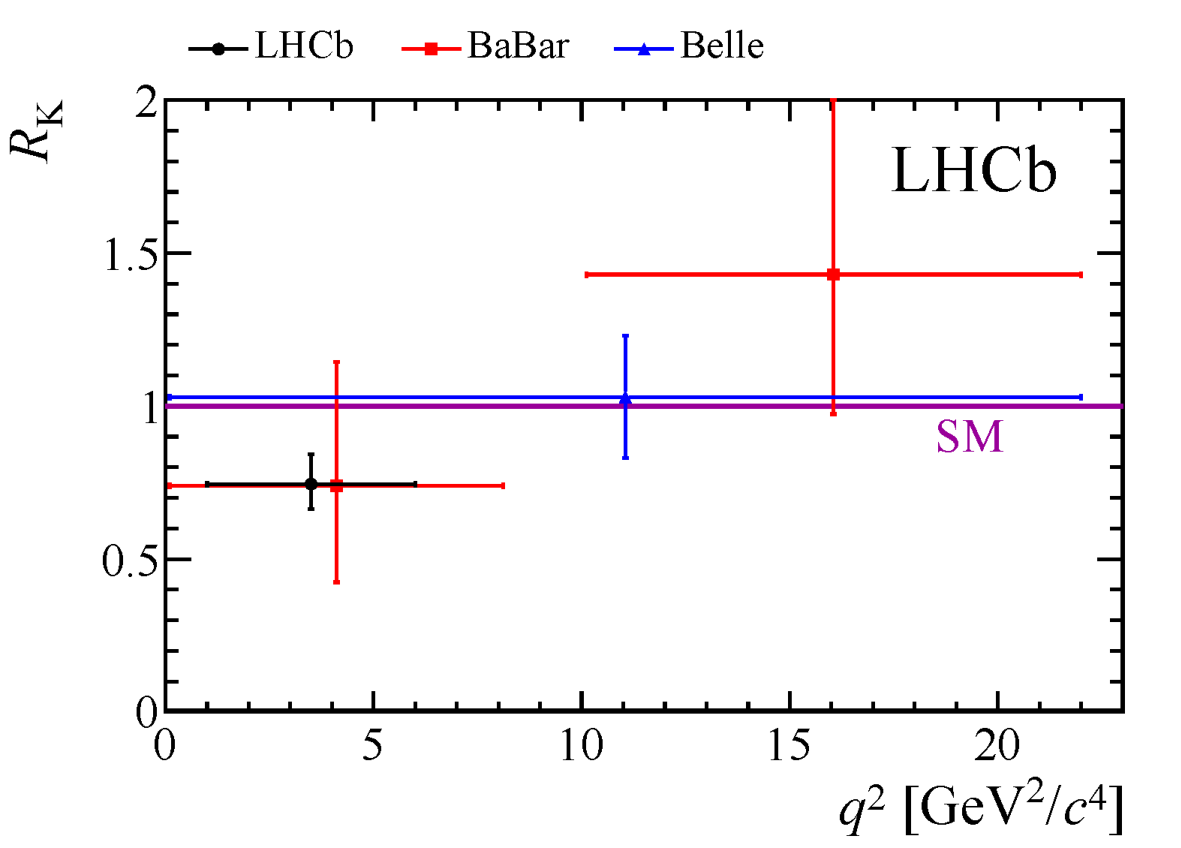
\includegraphics[width=7.5cm]{RK.pdf}
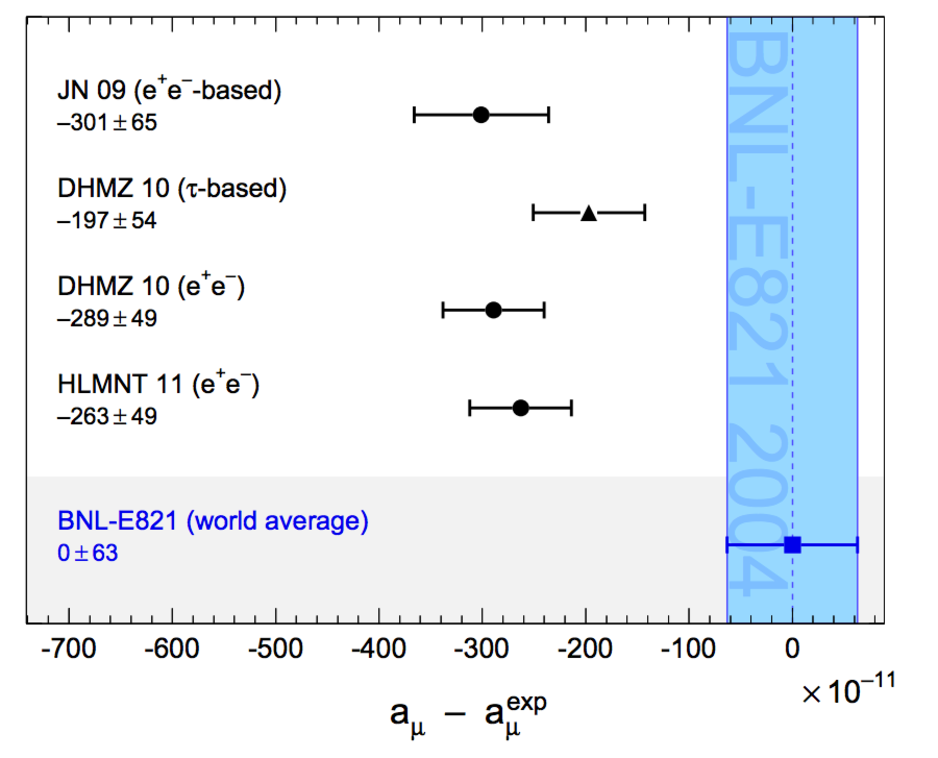
\includegraphics[width=7.5cm]{gminus2.pdf}
%\end{center}
\caption{Left plot: Measurements of the lepton universality observable $R_K$ from LHCb and the $B$-factories. The LHCb result at low $q^2$ exhibits a $2.6\sigma$ deviation from the SM prediction. Right plot:  Compilation from the PDG of recent published results
for $a_{\mu} = \frac{(g_{\mu}-2)}{2}$ 
(in units of $10^{-11}$), 
subtracted by the central value
of the 
experimental
 average.
 }
 \label{quarklep}
 \end{figure}
% 
%\label{quarklep}
%\end{figure}


From a theoretical point of view, it is also important to stress that
certain well motivated constructions called upon to address the quark flavour
puzzle have unavoidable implications regarding lepton flavours as
well. 
Examples of such constructions include extended Higgs sectors
(e.g., several realizations of 2HDM, type II seesaw, ...),
extended gauge sectors 
(e.g., additional $Z^\prime$ bosons) or additional symmetries  (flavour
symmetries, or gauge ones, such as left-right symmetric models), and finally 
larger frameworks as general Supersymmetry, extra dimensional models and
Grand Unified Theories. 

In all cases, it is clear that one must 
carefully evaluate the possible contributions to the
distinct charged lepton flavour observables: these include 
purely leptonic processes, such as 
radiative $\ell_i \to \ell_j \gamma$, 3-body $\ell_i \to 3\ell_j$,
etc., or processes involving hadron as is the case of semileptonic 
tau decays (such as $\tau \to \ell_i$+light hadrons), leptonic and 
semileptonic $B$, $D$
and $K$ meson decays,  and finally Higgs and $Z$ flavour violating
decays.
The expected contributions must be 
confronted with the available and soon to
be improved bounds, which will further allow to constrain the
parameter space of different theoretical models, possibly
impacting on the associated predictions regarding flavour
violation in the hadron sector. 
The synergy between the observables might allow to 
readily exclude some of these well motivated scenarios, and 
possibly to discriminate among distinct realizations of 
flavour violating models  (see, e.g.,~\cite{Abada:2014cca,Abada:2015zea,Abada:2015oba}). 

It is important to stress that the
studies above referred to 
will also have a natural impact on other flavour conserving 
observables, as is the case of the muon anomalous magnetic moment
$(g-2)_\mu$  (see figure~\ref{quarklep} right for the current status) 
or electric dipole moments of leptons. The exploration of these observables, foreseen in this GDR, might offer 
additional insights into the lepton and quark flavour puzzle.


\subsection*{Plans for the GDR}

Considering the interplay between quark and lepton flavour
violation, combining the informations and data arising from each
sector, is not only relevant but even mandatory to fully understand 
the underlying theory of flavour, and constrain, or even identify, 
the NP model at its origin. The GDR of the intensity frontier  will be a unique opportunity to share the competences in the quark and lepton sectors and to fully exploit this interplay. 


%% %%%%%%%%%%%%%%%%%%%%%%

